\section{Méthode}

\begin{figure}[H]
    \centering
    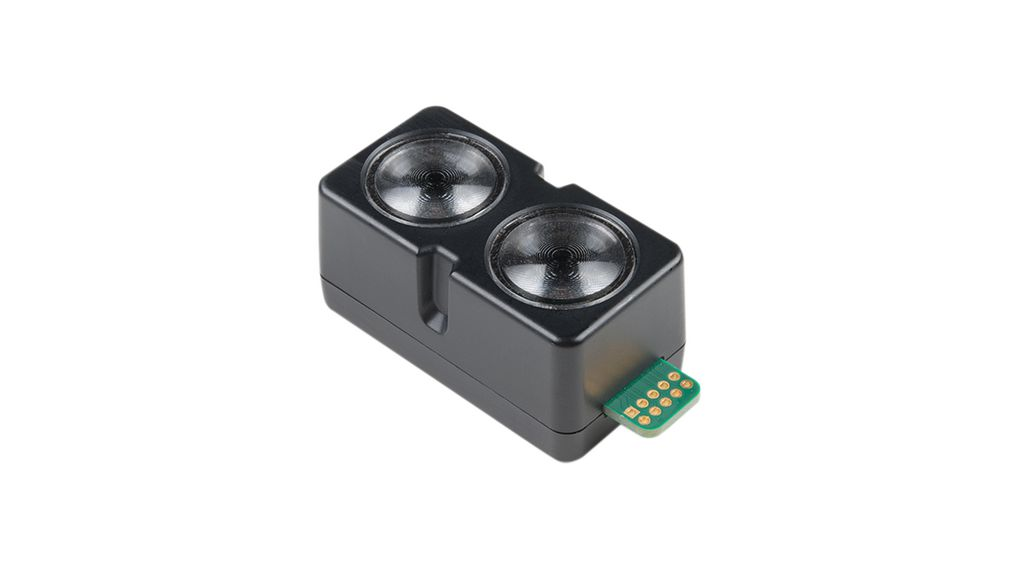
\includegraphics[width=0.5\textwidth]{Images/LiDAR/GarminLiDARLiteV4.jpg}
    \caption{Garmin Lidar Lite v4}
    \label{fig:LiDARLiteV4}
\end{figure}

Le LiDAR (ou \emph{laser imaging detection and ranging}) est un système de télédétection par laser,
utile pour mesurer des distances. Ce dernier envoie des faisceaux laser et mesure le temps du trajet
aller-retour vers le sujet. Il est ainsi possible de connaître avec plus ou moins de précision
quelle est la distance entre l'objet et le capteur.

\subsection{Fondamentaux}
Le LiDAR a l'avantage de mesurer des distances de manière non-intrusive. De cette manière, il n'y a 
aucun contact avec le milieu mesuré.\\
Dans le cadre du projet, cette solution est préférée car elle n'interfère pas avec la route et les 
machines de déneigement. Nous attendons donc que ce LiDAR mesure une hauteur de neige sur un 
segment de route de manière fiable, et ce à une distance d'environ 2 mètres du sol afin de protéger 
les instruments.\\
À partir d'une mesure de référence au sol, le capteur doit être capable de mesurer une hauteur de neige
présente dès les premières chutes, même après déneigement de la route. De plus, les conditions
météorologiques extrêmes présentes en altitude ne doivent en aucun cas perturber ces mesures, et ce
durant tout l'hiver. Finalement, il serait important de ne pas avoir à entretenir ou dépanner le système
au cours de la saison, sauf en cas de force majeure.\\
Lors d'une mesure, lorsqu'il neige, les flocons peuvent passer devant le capteur et interférer avec la
mesure. De ce fait, une solution efficace devra être développée afin de pouvoir mesurer efficacement
la hauteur de neige présente sur la route. De plus, le bruit généré par ces flocons pourra éventuellement
nous donner des informations sur le débit de neige actuel.

\subsection{Caractéristiques}
Après une étude détaillée des solutions disponibles sur le marché, nous avons retenu le LiDAR Lite V4
de la firme Garmin.\\
Il a l'avantage principal d'être livré dans un boîtier adapté (comme le montre la figure 
\ref{fig:LiDARLiteV4}), permettant une implémentation mécanique simple et rapide. Il faut cependant se 
méfier du fait que ce boîtier n'est pas étanche et ne peut par conséquent par être directement utilisé
en extérieur.

\begin{table}[H]
    \centering
    \begin{tabular}{|c|c|}
        \hline
        Specification & Measure \\
        \hline\hline
        Operating temperature   &   -20 to 60°C             \\
        \hline
        Operating voltage       &   4.75 to 5.25V           \\
        \hline
        Current consumption     &   2mA idle                \\
                                &   85mA during acquisition \\
        \hline
        Signals voltage         &   3.3V typical            \\
        \hline
        Range                   &   5cm to 10m               \\
        \hline
        Resolution              &   1cm                     \\
        \hline
        LED wavelength          &   940nm                   \\
        \hline
        Interface               &   I2C or ANT              \\
        \hline
        Update rate             &   I2C: Greater than 200Hz typical \\
        \hline
        Measurement 
        repeatability           &   \textpm 1cm to 2m       \\
                                &   \textpm 2cm to 4m       \\
                                &   \textpm 5cm to 10m      \\
        \hline
    \end{tabular}
    \caption{Extrait des spécifications du LiDAR Lite V4}
    \label{table:LiDARSpecs}
\end{table}

La table \ref{table:LiDARSpecs} montre une sélection des caractéristiques importantes du capteur, tirées
directement de sa fiche technique\footnote{Fiche technique du LiDAR Lite V4 :
\url{https://www.distrelec.ch/Web/Downloads/_m/an/SEN-15776_eng_man.pdf}}.
Ci-dessous sont détaillés les éléments essentiels à la sélection de ce capteur.

\begin{description}
    \item[Température de fonctionnement] \hfill \\ 
    Cette information s'avère importante pour ce projet. En
    effet, on peut s'attendre à ce que ce capteur puisse fonctionner à des températures négatives,
    allant jusqu'à -20°C. La borne supérieure de cette caractéristique nous intéresse moins, car
    ce sont des températures difficilement atteignables en hiver, même dans un boîtier fermé en 
    plein soleil.
    \item[Consommation de courant] \hfill \\ 
    Cette valeur est cruciale pour un projet qui se veut basse
    consommation et autonome. En effet, nous ne pouvons pas nous permettre de consommer plus que
    quelques microampères lorsque le système est en veille.\\
    Ainsi, on remarque que le capteur au repos consomme un courant relativement élevé de 2mA, ce
    qui n'est malheureusement pas acceptable. Pour cela, un système de déclenchement devra être
    implémenté (grâce à un MOSFET par exemple) afin de faire tomber cette consommation à zéro.\\
    Le courant de 85mA lorsque le LiDAR fait des acquisitions ne pose pas problème car la période 
    de mesure représente une partie négligeable du temps de fonctionnement total.
    \item[Tension des signaux] \hfill \\ 
    Il est important de noter que les signaux qui sont transmis au
    capteur (par le biais du bus I2C ou par les GPIO) doivent absolument avoir une tension de 3.3V.
    \item[Gamme de mesure] Le capteur est théoriquement capable de mesurer avec plus ou moins de
    précision n'importe quelle distance entre 5cm et 10m, ce qui satisfait entièrement les besoins
    du projet.
    \item[Longueur d'onde de la LED] \hfill \\ 
    Pour effectuer ses mesures, le LiDAR envoie des rayons lumineux
    infrarouges (940nm) grâce à une LED. Ainsi, compte tenu de la puissance du système et des limitations
    introduites par ce type de lumière, on peut d'ores et déjà s'attendre à ce que ce capteur ne
    fonctionne pas durant la journée.
    \item[Répétabilité des mesures] \hfill \\ 
    Cette information est nécessaire pour ajuster nos attentes quant
    à la précision attendue de ce capteur. Sur le terrain, il est estimé qu'il aura des distances 
    maximales de 3 mètres à mesurer, impliquant une précision typique de \textpm 2cm. 
\end{description}

De plus amples tests seront nécessaires pour attester de la véracité de ces informations sur le
terrain. Ils seront détaillés dans la section correspondante.

\subsection{Implémentation}

\begin{figure}[H]
    \centering
    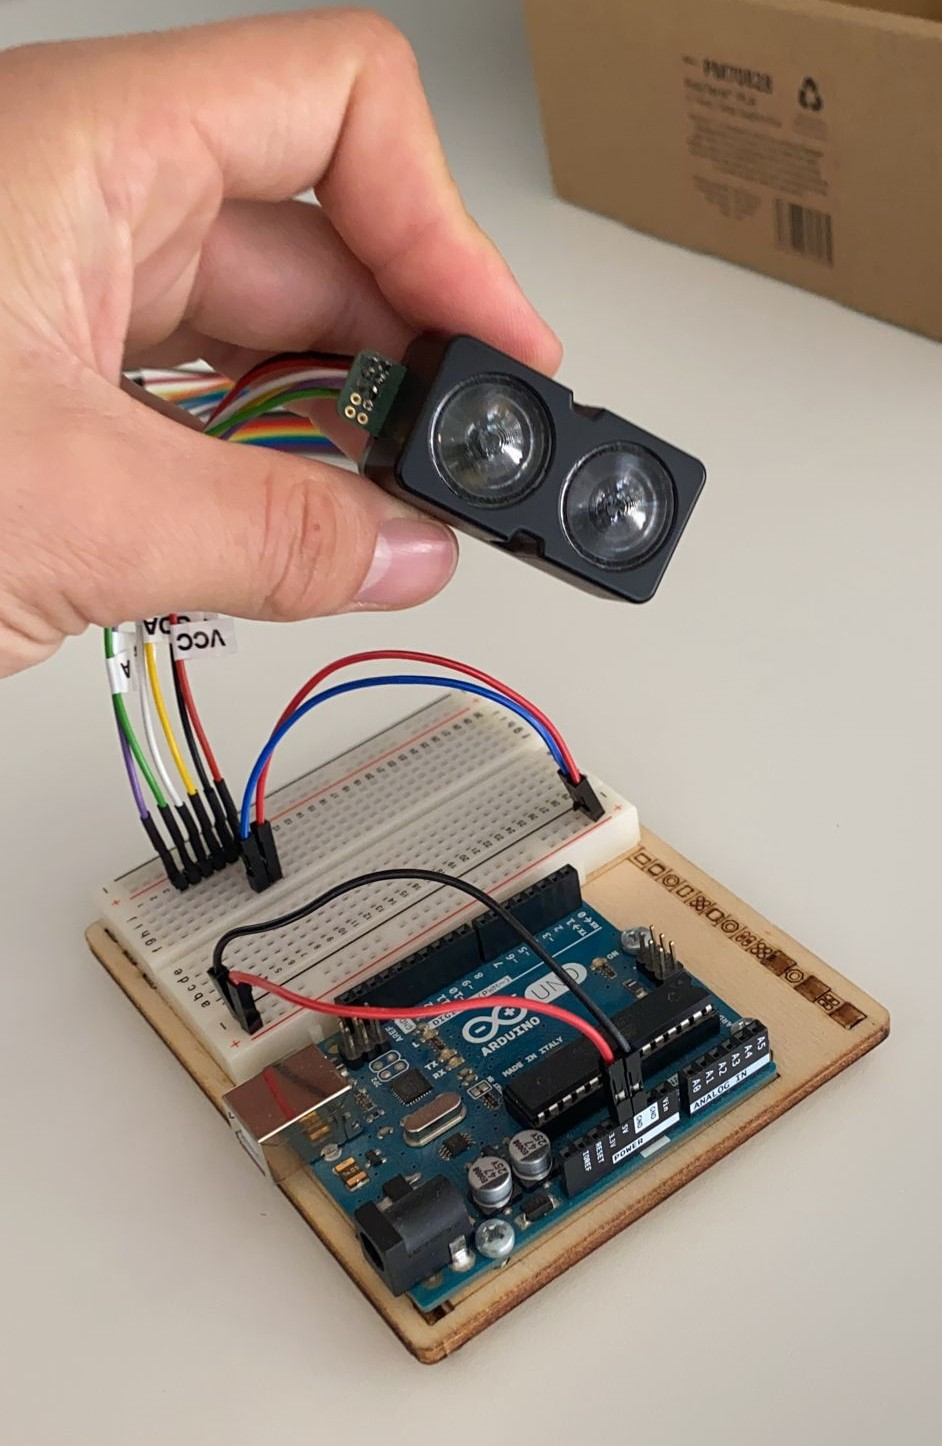
\includegraphics[width=0.4\textwidth]{Images/LiDAR/LiDAROnArduino.jpeg}
    \caption{LiDAR Lite V4 implémenté sur Arduino Uno}
    \label{fig:LiDAROnArduino}
\end{figure}

Afin d'implémenter le LiDAR avec un microcontrôleur, il a été choisi d'utiliser l'interface I2C
mise à disposition. Ce protocole est relativement simple à mettre en place et permet un bon débit de
donnée.\\
En plus des pins d'alimentation et de transmission I2C, le capteur met à disposition deux ports GPIO,
dénommés \emph{GPIOA} et \emph{GPIOB}. \emph{GPIOA} permet de déclencher une mesure du capteur sans
passer par la modification des registres I2C. \emph{GPIOB} informe le microcontrôleur de l'état actuel
de l'acquisition de mesures, et peut donc être configurée en interruption si nécessaire (état bas, prêt;
état haut, occupé).\par
Pour tester simplement et efficacement ce capteur, il a tout d'abord été interfacé sur Arduino Uno
à l'aide de la librairie Sparkfun fournie (voir figure \ref{fig:LiDAROnArduino}). Les premiers résultats 
sont détaillés dans la section correspondante.\\
Le capteur a été ensuite porté sur une carte de développement \emph{STM32F411RE NUCLEO} de la firme 
STMicroelectronics (figure \ref{fig:LiDAROnNUCLEO}) pour plus de flexibilité et une puissance de calcul plus importante. La libraire
mentionnée ci-dessus a été adaptée pour correspondre à l'environnement de développement dans le language
C.

\begin{table}[H]
    \centering
    \begin{tabular}{|c|c|m{7cm}|}
        \hline
        Register Address & Register Name & Value / Description \\
        \hline\hline
        0x00 & Device command & Write 0x04 : Take distance measurement with receiver bias \\
        \hline
        0x01 & System status & Read 0x00 : Busy flag (Low, ready; High, busy) \\
        &&                     Other values : See datasheet \\
        \hline
        0x10 & Distance measurement & Measured distance in cm \\ &Low byte& \\
        \hline
        0x11 & Distance measurement & Measured distance in cm \\ &High byte& \\
        \hline
    \end{tabular}
    \caption{Sélection des registres I2C essentiels}
    \label{table:LiDARI2C}
\end{table}

Dans le but de prendre des mesures de distance, plusieurs registres I2C doivent être consultés. La
table \ref{table:LiDARI2C} montre une sélection de 4 registres essentiels au fonctionnement de ce capteur.
Premièrement, une commande de mesure de distance est envoyée dans le registre 0x00, puis on attend
grâce au status (0x01) que l'appareil ne soit plus occupé. Les deux registres 0x10 et 0x11 peuvent ensuite
être consulté afin de recomposer une valeur 16 bits représentant la distance mesurée, en centimètre.\\
Par défaut, le LiDAR possède une adresse I2C fixée à 0x62.

\begin{figure}[H]
    \centering
    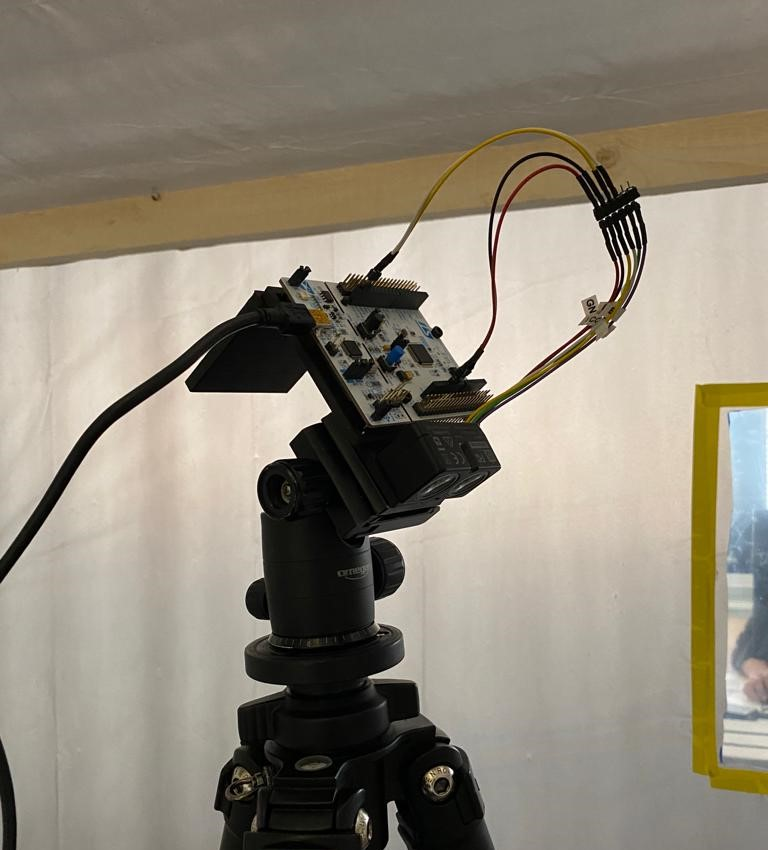
\includegraphics[width=0.5\textwidth]{Images/LiDAR/LiDAROnNucleo.jpeg}
    \caption{LiDAR Lite V4 sur STM32-NUCLEO}
    \label{fig:LiDAROnNUCLEO}
\end{figure}
\newpage

\subsection{Méthode de mesure}
\label{sec:MethodeDeMesure}

Une méthode de mesure de hauteur de neige doit être établie avant de poursuivre le développement. Comme
le capteur sera placé en bordure de route à un angle connu de la verticale, un peu de trigonométrie est
nécessaire afin de retrouver une hauteur de neige avec deux mesures de distances. La situation est
schématisée sur la figure \ref{fig:LiDARMesMethod}.

\begin{figure}[H]
    \centering
    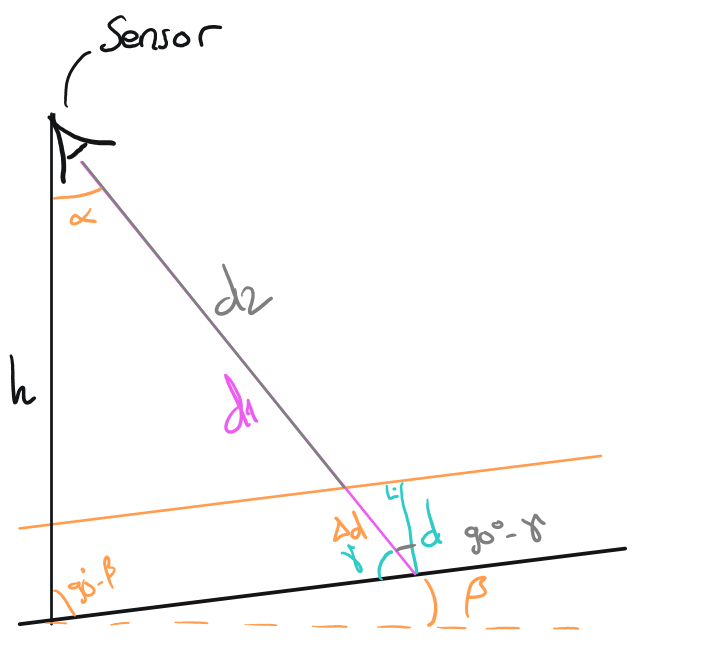
\includegraphics[width=0.5\textwidth]{Images/LiDAR/LiDAR_MesMethod.png}
    \caption{Schéma de l'installation d'un module LoRaSnow}
    \label{fig:LiDARMesMethod}
\end{figure}

\begin{description}
    \item[$\alpha$] Angle du capteur par rapport à la verticale (en degré)
    \item[$\beta$] Angle du segment de route mesuré par rapport à l'horizontale (en degré)
    \item[$\gamma$] Angle entre le faisceau du LiDAR et le segment de route (en degré) 
    \item[$d_1$] Distance de référence entre le capteur et le segment de route (en centimètre)
    \item[$d_2$] Distance mesurée entre le capteur et une hauteur de neige (en centimètre)
    \item[$\Delta d$] Différence entre la distance de référence et la distance à la neige (en centimètre) 
    \item[$d$] Hauteur de neige sur la route (en centimètre) 
    \item[$h$] Distance entre le capteur et le sol, à la vertical (en centimètre)
\end{description}

Lors de l'installation du module, $\alpha$, $\beta$ et $h$ doivent être connus. Avec ces valeurs, on
peut désormais calculer facilement l'angle $\gamma$ :

\[\gamma = 180^{\circ} - 90^{\circ} + \beta - \alpha = 90^{\circ} + \beta - \alpha\]

Le $\Delta d$ est simplement la différence entre la distance de référence et la distance entre la
neige et le capteur :

\[\Delta d = d_1 - d_2\]

Ces deux informations nous permettent maintenant de déterminer la hauteur de neige présente sur le
segment de route mesuré :

\[d = \Delta d * \cos{(90^{\circ} - \gamma)}\]

Il est important de noter que la résolution du capteur est de 1 centimètre, ce qui implique que la
hauteur de neige mesurée va varier par pas de $\cos{(90^{\circ} - \gamma)}$.